\documentclass[a4paper,french,towsides,10pt]{book}
\usepackage[utf8]{inputenc}
\usepackage[french]{babel}
\usepackage{fancyhdr}
\usepackage{enumerate}
\usepackage{graphicx}
\usepackage{multirow}
\usepackage{placeins}
\usepackage{tabularx}
\usepackage[french,ruled,vlined,linesnumbered]{algorithm2e}
\usepackage{amsmath}
\usepackage{amssymb}
\usepackage[bookmarks=true]{hyperref}
\hypersetup{pdfborder={0 0 0}}
\pagestyle{fancy}
\setlength{\parskip}{1.5ex plus .4ex minus .4ex}
\renewcommand{\labelitemi}{\textbullet}
\renewcommand{\chaptermark}[1]{\markboth{#1}{}}



\pagestyle{fancy}

\renewcommand{\chaptermark}[1]{\markboth{#1}{}}
\renewcommand{\sectionmark}[1]{\markright{\thesection\ #1}}

\fancyhf{}

\fancyhead[RO,LE]{\thepage}
\fancyhead[LO]{\leftmark}
\fancyhead[RE]{Projet GMIN103 Base de données avancée}

\fancypagestyle{corps}{ 
\fancyhead[RO,LE]{\thepage}
\fancyhead[LO]{\rightmark}
\fancyhead[RE]{\leftmark}
}

\renewcommand{\footrulewidth}{0pt} % pas de filet en bas
\fancypagestyle{plain}{ % pages de tetes de chapitre
\fancyhead{}
% supprime l’entete
\renewcommand{\headrulewidth}{0pt} % et le filet
}
\newcommand{\clearemptydoublepage}{%
	\newpage{\pagestyle{empty}\cleardoublepage}}


%Modification des marges
%\\oddsidemargin}{-2,5cm}
%\addtolength{\textwidth}{5cm}
%\addtolength{\topmargin}{-2,5cm}
%\addtolength{\textheight}{4cm}

%definition des fonctions de la page de garde
\input{includes/gardedef}

%definition du titre et autres param
\def\titre{\LARGE Projet GMIN103 Base de données avancée \\ Thésaurus}
\def\sstitre{Rapport (Décembre 2011)}
\def\auteurs{
	  Baptiste \textsc{Le Bail} \\
      Thibaut \textsc{Marmin} \\
      Namrata \textsc{Patel} \\
      Clément \textsc{Sipieter} \\
      Steeve \textsc{Tuvée}}

\begin{document}
\frontmatter
\renewcommand{\labelitemii}{\textasteriskcentered}
\thispagestyle{empty}
  \vbox to .9\vsize{%
  \vss
  \vbox to 1\vsize{%
    \haut{}{\blurb}{}
    \vfill
    
    \noindent\rule{\linewidth}{.5pt}
    \ligne{\vspace{1.5mm}\titre}
    \noindent\rule{\linewidth}{.5pt}
    \ligne{\normalsize{\textsc{\sstitre}}}
    \vfill
    \ligne{%
      \begin{tabular}{l}
	\vspace{5mm}
      \end{tabular}
      \begin{tabular}{c}
      Travail réalisé par : \\\\
       \auteurs
      \end{tabular}
    }
  \vss
  }
}
\clearemptydoublepage
\chapter*{Introduction}
Un thésaurus est un type de langage documentaire qui constitue un vocabulaire normalisé. Il regroupe de manière organisée les termes d'un même domaine de connaissance. Cet outil linguistique permet de décrire des concepts et de lever les ambiguïtés induites par les relations de synonymie, d'homonymie et de polysémie présentes dans le langage naturel.

L'outil développé lors de ce projet sera composé de termes décrivant des concepts, reliés entre eux par des relations hiérarchiques, synonymiques et associatives. L'utilisateur aura la possibilité d'explorer la hiérarchie et de gérer (ajouter / modifier / supprimer) les termes et les concepts.

Ce travail, réalisé par une équipe de cinq étudiants\footnote{Baptiste Le Bail, Thibaut Marmin, Namrata Patel, Clément Sipieter, Steeve Tuvée}, est présenté dans ce rapport selon trois phases distinctes : analyse, conception, implémentation.
\clearemptydoublepage
\tableofcontents
\clearemptydoublepage
\mainmatter
\chapter{Analyse}
\textit{La phase d'analyse est un élément indispensable à la bonne réalisation du projet. Dans un premier temps, les fonctionnalités de l'application y sont décrites et caractérisées, notamment à l'aide d'un diagramme UML de cas d'utilisations. Une seconde partie présente les étapes successives qui nous ont permis d'arriver à la modélisation finale, sous la forme de diagrammes UML de classes et de \og{}discussions\fg{}.}

\section{Fonctionnalités}

L'application devra modéliser un thésaurus stocké dans une base de données, et devra permettre sa consultation au travers d'une interface web. L'utilisateur pourra donc consulter ou administrer les données. La consultation du thésaurus se fera par navigation dans une vue hiérarchique ou par nœud. Un outil de recherche facilitera l'accès aux données. Le module d'administration permettra quand à lui d'ajouter, de modifier et de supprimer les termes et les concepts, ainsi que les relations.

\begin{figure}[H]
\begin{center}
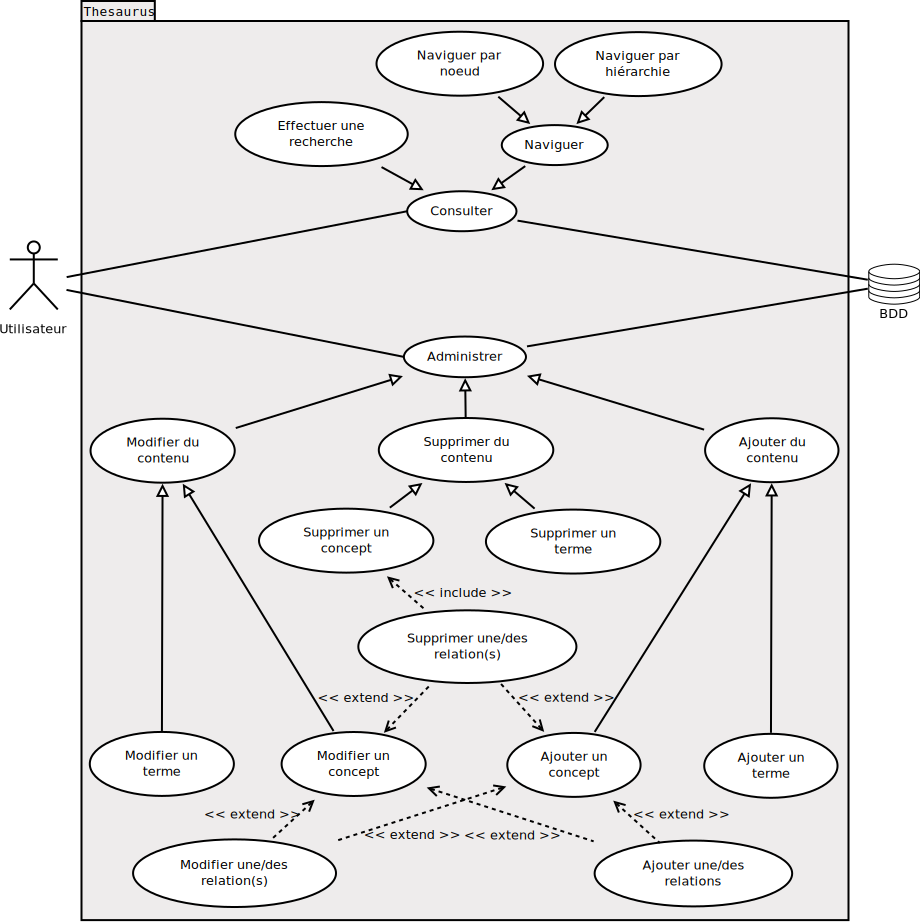
\includegraphics[width=\textwidth]{files/usecase}
\end{center}
\caption{Diagramme de cas d'utilisations}
\end{figure}

\section{Modélisation} 

Un thésaurus est composé de deux types d'entités : les Termes et les Concepts.
\begin{description}
\item[Concepts] : ils sont décrits par un descripteur (terme vedette), et sont organisés hiérarchiquement par relations de concepts généraux (parents) et spécifiques (fils). Les concepts peuvent aussi être mis en relation par simple association.
\item[Termes] : ils sont définis par un libellé et sont en relation de synonymie entre eux.
\end{description}

\subsection{Une première piste...}
Pour notre première modélisation, nous avons fait le choix de respecter la définition stricte du thésaurus rappelée ci-dessus.

\begin{figure}[H]
\begin{center}
\includegraphics[width=0.8\textwidth]{files/class_v1}
\end{center}
\caption{Première version du diagramme de classes.}
\end{figure}

Bien que la définition soit rigoureusement respectée, cette modélisation est limitée : il est impossible de lever le problème de polysémie sur les termes. En effet prenons le terme \og avocat \fg. Celui-ci peut désigner un fruit ou un métier. La relation de synonymie est donc ambigüe bien que cette modélisation permet la création de deux concepts ayant comme le même terme vedette.

\subsection{Évolution}
Pour résoudre ce problème d'ambiguïté des synonymes, il est nécessaire de distinguer ce type de relation en ajoutant une dépendance à un concept.

\begin{figure}[H]
\begin{center}
\includegraphics[width=0.8\textwidth]{files/class_v2}
\end{center}
\caption{Évolution du diagramme de classes.}
\end{figure}

Ce modèle est légèrement éloigné de la définition d'un thésaurus car les termes ne sont plus en relation de synonymie entre eux, mais avec des concepts. Nous avons donc choisi de spécialiser la classe Terme en deux classes filles \texttt{TermeVedette} et \texttt{TermeSynonyme}. Un concept est maintenant décrit à la fois par plusieurs termes : un terme vedette de type \texttt{TermVedette} et des synonymes de type \texttt{TermeSynonyme}.

\subsection{Décision finale}

Pour cette dernière étape de réflexion, nous avons choisi de simplifier la modélisation.

\begin{figure}[H]
\begin{center}
\includegraphics[width=\textwidth]{files/class_v3}
\end{center}
\caption{Version finale du diagramme de classes.}
\end{figure}

La suppression de l'héritage de terme nous rapproche du modèle initial, tout en conservant la résolution du problème lié à la polysémie. En effet, la distinction entre les termes vedette et les termes synonymes peut être ignorée.

Reprenons le problème de l'\og avocat \fg : le terme sera stocké une fois en base, mais sera terme vedette de deux concepts : celui d'\og avocat \fg le fruit, et celui d'\og avocat \fg le métier. Le premier concept (fruit) pourra ne contenir aucun synonyme, tandis que le deuxième concept pourra avoir comme synonyme \og défenseur \fg{}.
\chapter{Conception}
Schéma objet-relationnel / 100\% relationnel.

Discussion sur pourquoi 100\% relationnel ?! ORM ?! Doctrine / Symfony ?

Présentation des templates / formulaires

\section{Objet-relationnel\ldots}

\section{Pourquoi un ORM ?}

\section{Décisions}
\subsection{Templates}
\subsection{Framework}
\chapter{Implémentation}
Classes réellement implémentées dans symfony2 + schema relationnel créé par doctrine.

Aperçus d'écran finaux

\section{Présentation de Symfony2}

\section{Entities implémentées}

\section{Schéma relationnel généré}

\section{Templates finaux}
\end{document}